\documentclass{scrarticle}

\usepackage{amsmath}
\usepackage{graphicx}

\title{\LaTeX}
\author{Einstein}

\begin{document}
\maketitle

\LaTeX{} is a document preparation system for the \TeX{} typesetting program. It offers programmable desktop publishing features and extensive facilities for automating most aspects of typesetting and desktop publishing, including numbering and  cross-referencing, tables and figures, page layout, bibliographies, and much more. \LaTeX{} was originally written in 1984 by Leslie Lamport and has become the  dominant method for using \TeX; few people write in plain \TeX{} anymore. The current version is \LaTeXe.

\begin{align}
E_0 &= mc^2 \\
E &= \frac{mc^2}{\sqrt{1-\frac{v^2}{c^2}}}
\end{align}

\begin{figure}[htbp]
\centerline{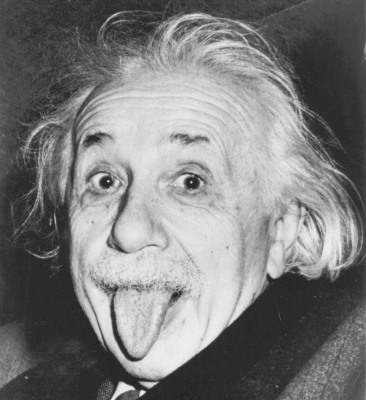
\includegraphics[width=0.3\linewidth]{einstein}}
\caption{Example of a figure caption.}
\label{fig}
\end{figure}

\end{document}
